% !TEX root = main.tex
\subsubsection{Contextual linear Gaussian bandits}
\label{sssec:evaluation_contextual_linear_baselines}

We first investigate the performance of our proposed method in the classic contextual linear Gaussian MAB setting: \ie for bandits where rewards are drawn from linearly parameterized arms, where the mean reward for context $x_t$ and arm $a$ is given by $x_t^\top \theta_a$, for some unknown latent parameter $\theta_a$.

We evaluate different parameterizations of such bandits, both for non-sparse and sparse settings (where only few components of $\theta_a$ are non-zero for each arm).
Specifically, we draw a 10 dimensional $\theta_a$ uniformly at random (with only 3 components left as non-zero for each arm in the sparse setting), with contexts distributed as a 10-dimensional standard Gaussian. In all cases, Gaussian noise (with a minimum standard deviation of 0.01) is added to the rewards of each arm, for $|\mathcal{A}|=8$.

Figures~\ref{fig:linear_showdown_baselines_top_regret} and~\ref{fig:sparse_linear_showdown_baselines_top_regret} showcase the five top performing algorithms in non-sparse and sparse linear contextual bandits respectively, with cumulative regret results (and attained relative regret improvements) detailed in Tables~\ref{tab:linear_showdown_baselines_regret} and \ref{tab:sparse_linear_showdown_baselines_regret} for all the evaluated methods.
The corresponding reward results are provided in Section~\ref{asec:linearGaussian_baselines} of the Appendix.

% Linear Gaussian regret figure
\begin{figure}[!ht]
	\centering
	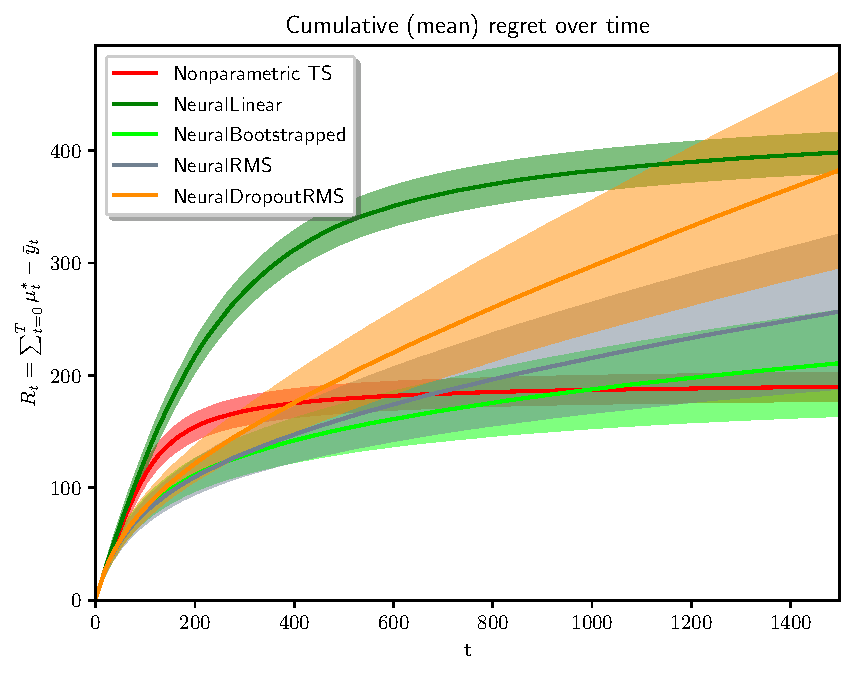
\includegraphics[width=0.75\textwidth]{./figs/linear_showdown_baselines/cum_optexpected_regret_top_five_std}
	\vspace*{-5ex}
	\caption{Mean regret (standard deviation shown as shaded region) for $R=500$ realizations of the presented methods in contextual linear Gaussian MABs.}
	\label{fig:linear_showdown_baselines_top_regret}
	\vspace*{-2ex}
\end{figure}
% Linear Gaussian regret figure
\begin{table}[!h]
	\caption{Cumulative regret at $t=1500$ for $R=500$ realizations of contextual linear Gaussian MABs. The second column showcases the additional relative cumulative regret incurred by each algorithm when compared to \texttt{Nonparametric TS} at $t=1500$.}
	\label{tab:linear_showdown_baselines_regret}
	\vspace*{-4ex}
	\begin{center}
		\resizebox*{0.75\textwidth}{!}{
			\begin{tabular}{|c|c|c|}
				\hline
				Algorithm 	\cellcolor[gray]{0.6} & Cumulative regret \cellcolor[gray]{0.6} & Relative cumulative regret \cellcolor[gray]{0.6} \\ \hline
				Nonparametric TS     	 & 189.889 & \%0.000 \\ \hline
				NeuralLinear         	 & 398.485 & \%109.852 \\ \hline
				NeuralBootstrapped   	 & 210.914 & \%11.073 \\ \hline
				NeuralRMS            	 & 256.897 & \%35.288 \\ \hline
				NeuralDropoutRMS     	 & 382.870 & \%101.629 \\ \hline
				NeuralParamNoise     	 & 241.039 & \%26.937 \\ \hline
				MultitaskGP          	 & 213.648 & \%12.512 \\ \hline
				BNNVariationalGaussian 	 & 827.369 & \%335.712 \\ \hline
				BNNAlphaDiv          	 & 793.118 & \%317.675 \\ \hline
			\end{tabular}
		}
	\end{center}
	\vspace*{-2ex}
\end{table}

We observe a reduced cumulative regret of our proposed nonparametric Thompson sampling when compared to all state-of-the-art Thompson sampling alternatives described in Section~\ref{ssec:ts_baselines}.
The proposed \texttt{Nonparametric TS} method achieves logarithmic regret, even as it estimates the true form of the underlying unknown reward function, resulting in considerably smaller regret than the alternatives ---designed to be flexible for complex bandit scenarios--- in the contextual linear Gaussian setting.

The neural network based linear Thompson sampling method (\ie \texttt{NeuralLinear}) achieves logarithmic regret as well, but suffers an important loss: an average cumulative regret that doubles that of \texttt{Nonparametric TS} at $t=1500$.

% Sparse Linear Gaussian regret figure
\begin{figure}[!ht]
	\vspace*{-2ex}
	\centering
	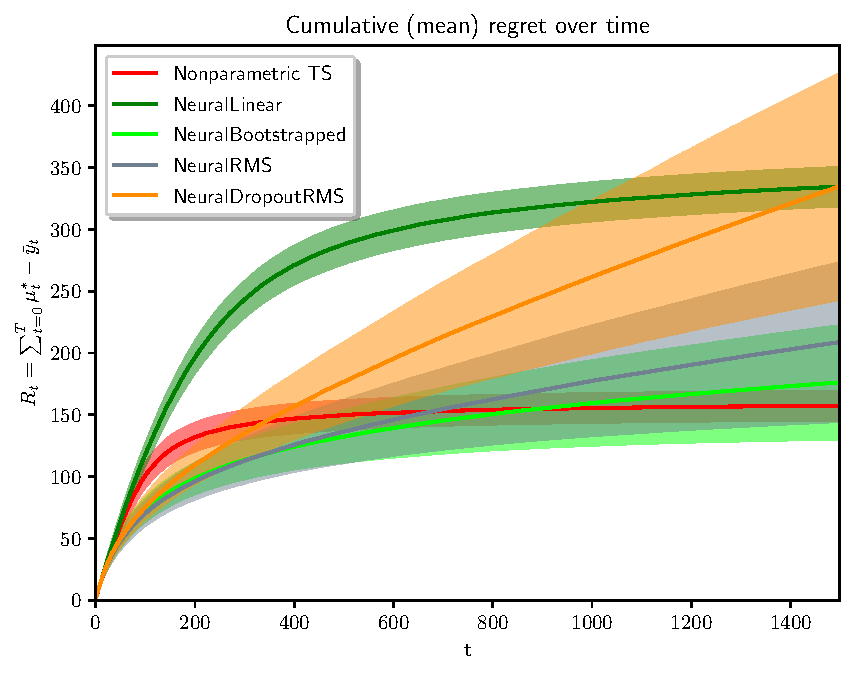
\includegraphics[width=0.75\textwidth]{./figs/sparse_linear_showdown_baselines/cum_optexpected_regret_top_five_std}
	\vspace*{-5ex}
	\caption{Mean regret (standard deviation shown as shaded region) for $R=500$ realizations of the presented methods in sparse contextual linear Gaussian MABs.}
	\label{fig:sparse_linear_showdown_baselines_top_regret}
	\vspace*{-2ex}
\end{figure}
% Sparse Linear Gaussian regret table
\begin{table}[!h]
	\caption{Cumulative regret at $t=1500$ for $R=500$ realizations of sparse contextual linear Gaussian MABs. The second column showcases the additional relative cumulative regret incurred by each algorithm when compared to \texttt{Nonparametric TS} at $t=1500$.}
	\label{tab:sparse_linear_showdown_baselines_regret}
	\vspace*{-4ex}
	\begin{center}
		\resizebox*{0.75\textwidth}{!}{
			\begin{tabular}{|c|c|c|}
				\hline
				Algorithm 	\cellcolor[gray]{0.6} & Cumulative regret \cellcolor[gray]{0.6} & Relative cumulative regret \cellcolor[gray]{0.6} \\ \hline
				Nonparametric TS     	 & 157.406 & \%0.000 \\ \hline
				NeuralLinear         	 & 334.569 & \%112.551 \\ \hline
				NeuralBootstrapped   	 & 176.136 & \%11.899 \\ \hline
				NeuralRMS            	 & 208.738 & \%32.611 \\ \hline
				NeuralDropoutRMS     	 & 334.870 & \%112.742 \\ \hline
				NeuralParamNoise     	 & 199.122 & \%26.502 \\ \hline
				MultitaskGP          	 & 186.023 & \%18.180 \\ \hline
				BNNVariationalGaussian 	 & 762.321 & \%384.301 \\ \hline
				BNNAlphaDiv          	 & 695.097 & \%341.594 \\ \hline
				
			\end{tabular}
		}
	\end{center}
	\vspace*{-2ex}
\end{table}

Bootstrapped and RMS based alternatives fail to achieve a good exploration-exploitation trade-off (their cumulative regret does not plateau by $t=1500$), with cumulative regrets that are at least 10\% and 30\% higher in all contextual MABs.
In addition, their performance is highly volatile across realizations of the same problem (recall their wide shaded regions in Figures~\ref{fig:linear_showdown_baselines_top_regret} and~\ref{fig:sparse_linear_showdown_baselines_top_regret}).
Specially concerning is the poor performance of all the Bayesian Neural Network (BNN) based baselines, which incur in more than \%300 cumulative regret increase with respect to \texttt{Nonparametric TS}.

These results support our claim that a nonparametric Bayesian based Thompson sampling is a flexible alternative that can provide reduced regret when compared to state-of-the-art baselines.